\documentclass{article}
\usepackage{amsmath}
\usepackage{booktabs}
\usepackage{geometry}
\usepackage{graphicx}
\usepackage{grffile}
\geometry{a4paper, margin=1in}

\title{Physics-Informed SINDy Parameter Recovery and Validation for Coupled Nonlinear Viscoelasticity}
\author{Data Driven Project Team}
\date{June 26, 2026}

\begin{document}

\maketitle

\section{Introduction and Physical Derivation}
This document summarizes the methodology, physical derivation, parameter recovery, and validation results for the 3D coupled nonlinear viscoelastic Maxwell model using Sparse Identification of Nonlinear Dynamics (SINDy) in deviatoric space.

To represent shape-changing viscous flow in isotropic materials, the model is formulated in deviatoric stress and strain rate spaces. The step-by-step physical derivation is detailed below.

\subsection{Step 1: 1D Maxwell Viscoelastic Model}
The classical Maxwell model represents a viscoelastic material as an elastic spring and a viscous dashpot connected in series. The total strain rate ($\dot{\varepsilon}$) is the sum of the elastic strain rate ($\dot{\varepsilon}_{\text{elastic}}$) and the viscous strain rate ($\dot{\varepsilon}_{\text{viscous}}$):
\begin{equation}
    \dot{\varepsilon} = \dot{\varepsilon}_{\text{elastic}} + \dot{\varepsilon}_{\text{viscous}}
\end{equation}
Applying Hooke's law for the spring ($\sigma = 2G \varepsilon_{\text{elastic}}$) and Newton's law for the dashpot ($\sigma = \eta \dot{\varepsilon}_{\text{viscous}}$), we substitute the rates:
\begin{equation}
    \dot{\varepsilon} = \frac{1}{2G}\dot{\sigma} + \frac{\sigma}{\eta}
\end{equation}
Rearranging for the stress rate ($\dot{\sigma}$) yields the governing differential equation:
\begin{equation}
    \dot{\sigma} = 2G\dot{\varepsilon} - \frac{2G}{\eta}\sigma
\end{equation}

\subsection{Step 2: 3D Generalization in Deviatoric Space}
For a 3D isotropic material, volumetric changes are assumed elastic, whereas shape-changing (deviatoric) stress components $S_{ij}$ drive the viscous flow. Generalizing the 1D Maxwell equation to the deviatoric stress tensor $S_{ij}$ and the deviatoric strain rate tensor $\dot{\varepsilon}^{dev}_{ij}$ gives:
\begin{equation}
    \frac{dS_{ij}}{dt} = 2G\dot{\varepsilon}^{dev}_{ij} - \frac{2G}{\eta}S_{ij}
\end{equation}
where $G$ is the shear modulus and $\eta$ is the material viscosity.

\subsection{Step 3: Stress-Dependent Viscosity (J2 Flow Theory)}
In nonlinear viscoelasticity, viscosity is stress-dependent. To ensure physical isotropy (i.e., that the material's properties are frame-invariant and independent of the coordinate system), the viscosity must depend solely on the scalar invariants of the stress tensor. Since hydrostatic stress is removed, the simplest invariant for deviatoric stress is the second invariant $J_2 = 0.5 \mathbf{S} : \mathbf{S}$. This is directly proportional to the von Mises equivalent stress squared:
\begin{equation}
    \sigma_{eq}^2 = 3 J_2 = 1.5 \left( S_{xx}^2 + S_{yy}^2 + S_{zz}^2 + 2 S_{xy}^2 + 2 S_{yz}^2 + 2 S_{xz}^2 \right)
\end{equation}
We model the nonlinear softening (shear-thinning) viscosity $\eta(\sigma_{eq})$ using a Taylor expansion/power-law formulation:
\begin{equation}
    \frac{1}{\eta(\sigma_{eq})} = \frac{1}{\eta_0}(1 + \alpha \sigma_{eq}^2)
\end{equation}
where $\eta_0$ is the reference viscosity at zero stress and $\alpha$ is the nonlinear softening coefficient.

\subsection{Step 4: Coupled Constitutive Evolution Equations}
Substituting the stress-dependent viscosity model back into the 3D deviatoric Maxwell equation gives:
\begin{equation}
    \frac{dS_{ij}}{dt} = 2G\dot{\varepsilon}^{dev}_{ij} - 2G\left[ \frac{1}{\eta_0}(1 + \alpha \sigma_{eq}^2) \right]S_{ij}
\end{equation}
Distributing the stress tensor $S_{ij}$ yields the final system of coupled differential equations:
\begin{equation}
    \frac{dS_{ij}}{dt} = \underbrace{2G \dot{\varepsilon}^{dev}_{ij}}_{\text{Strain Rate Term}} - \underbrace{\frac{2G}{\eta_0} S_{ij}}_{\text{Linear Stress Term}} - \underbrace{\frac{2G\alpha}{\eta_0} (S_{ij} \sigma_{eq}^2)}_{\text{Nonlinear J2 Term}}
\end{equation}

---

\section{Physics-Informed SINDy Library Design}
The key challenge in data-driven discovery of material models is ensuring the optimizer converges to the correct physical structure. We compare a naive SINDy approach with our physics-informed library design.

\subsection{The Naive Approach (Polynomial Library Expansion)}
The nonlinear term $(S_{ij} \sigma_{eq}^2)$ is a cubic polynomial of the stress components (e.g., $S_{xx}^3$, $S_{xx}S_{yy}^2$, etc.). If we did not pre-compute this term, we would have to search for it using a general cubic polynomial library ($\text{degree} = 3$) on our 12 input variables (6 stresses + 6 strain rates). 

The number of candidate terms in a 12-variable cubic library is:
\begin{equation}
    N_{\text{candidates}} = \frac{(12 + 3)!}{12! \, 3!} = 455 \text{ terms per equation}
\end{equation}
Searching through a space of 455 candidates introduces severe issues:
\begin{itemize}
    \item \textbf{Loss of Sparsity}: With noise in the stress measurements, the optimizer will select incorrect terms that happen to fit the noise, losing physical interpretability.
    \item \textbf{Numerical Collinearity}: Many cubic terms are highly correlated during simple loading tests, causing the optimization problem to be ill-conditioned.
\end{itemize}

\subsection{The Physics-Informed Approach}
By calculating the invariant $\sigma_{eq}^2$ from the stress tensor components and multiplying it by each individual stress component, we pre-compute the J2 coupled stress tensor:
\begin{equation}
    Seq_{ij} = S_{ij} \sigma_{eq}^2
\end{equation}
We pass $Seq_{ij}$ directly to the SINDy library as a known control input variable. This reduces the library for each coordinate derivative $\frac{d S_{ij}}{dt}$ to a linear combination of just three candidate terms:
\begin{equation}
    \text{Library for } S_{ij} = \left\{ 1, \,\, S_{ij}, \,\, \dot{\varepsilon}^{dev}_{ij}, \,\, Seq_{ij} \right\}
\end{equation}
This reduces the search space from **455 terms to 3 terms**, guaranteeing that the optimizer fits the correct physical structure, handles noise robustly, and yields coefficients that map directly back to the physical parameters $G$, $\eta_0$, and $\alpha$.

---

\section{Methodology: Split Training vs. Coupled Validation}
To identify the parameters while ensuring multiaxial validity, we decoupled the training strategy from the validation simulation:

\begin{itemize}
    \item \textbf{Split Training (Resolving Collinearity)}: 
    The training datasets consist of standard, single-axis testing histories (uniaxial tension and pure shear). In these simple paths, components are perfectly collinear (e.g., $S_{yy} = S_{zz} = -0.5 S_{xx}$ in uniaxial tension). Fitting a 6D SINDy model directly on this data causes severe multicollinearity, prompting the optimizer to split coefficients arbitrarily across collinear terms. 
    
    To resolve this, we fit the equations component-by-component ($S_{xx}$ from uniaxial data, and $S_{xy}$ from shear data) using only their relevant candidate features (e.g. $ed_{xx}$ and $Seq_{xx}$). This isolates the independent physical coefficients and ensures exact parameter identification.
    
    \item \textbf{Coupled Validation (Evaluating Generalization)}: 
    In validation, we test the model on complex, unseen multiaxial loading paths (e.g. combined tension-shear and biaxial tension). Because the viscosity $\eta(\sigma_{eq})$ is a function of the second invariant $\sigma_{eq}^2$, all six stress components are physically coupled. 
    
    To calculate the viscosity at any given time step, the numerical solver must know all six stress components simultaneously. Therefore, we validate the model by integrating the six discovered equations together as a coupled 6D system of ordinary differential equations (ODEs).
\end{itemize}

\section{Addressing Reviewer Feedback}
A key feedback point raised by the reviewer on the linear model was:
\begin{quote}
    \textit{The multiaxial validation paths (Combined Uniaxial + Shear and Biaxial Tension) serve as multiaxial sanity checks under the isotropic assumption, but since the linear isotropic model decouples completely in deviatoric space, these paths represent the simple superposition of independent 1D trajectories rather than generalization to new nonlinear, coupled, or anisotropic constitutive behavior.}
\end{quote}

By implementing and fitting the J2-coupled nonlinear Maxwell model, we have successfully addressed this critique:
\begin{itemize}
    \item \textbf{True Multiaxial Coupling}: Because the viscosity $\eta(\sigma_{eq})$ depends on the stress invariant $\sigma_{eq}^2$ (which is a function of all stress components), the evolution of any component $S_{ij}$ depends nonlinearly on all other active stress components. The components do not decouple.
    \item \textbf{Generalization to Nonlinear Coupled Behavior}: The validation on combined loading (simultaneous uniaxial tension and shear) is not a linear superposition of 1D paths. It requires the model to correctly generalize to a coupled multiaxial state. 
    \item \textbf{Validation Success}: SINDy successfully recovers the coupling parameter $\alpha$ with $0.228\%$ error and predicts the response on unseen combined loading paths with high accuracy ($\text{RMSE} < 0.02\text{ MPa}$), showing robust generalization.
\end{itemize}

\section{Discovered SINDy Equations}
Using a component-by-component fitting strategy with an STLSQ sparsity threshold of $10^{-5}$, the following 3D coupled equations were discovered:
\begin{align*}
    \frac{d S_{xx}}{dt} &= 0.034 - 4.007 S_{xx} + 2000.845 \dot{\varepsilon}^{dev}_{xx} - 0.001 S_{xx} \sigma_{eq}^2 \\
    \frac{d S_{yy}}{dt} &= 0.034 - 4.007 S_{yy} + 2000.845 \dot{\varepsilon}^{dev}_{yy} - 0.001 S_{yy} \sigma_{eq}^2 \\
    \frac{d S_{zz}}{dt} &= 0.034 - 4.007 S_{zz} + 2000.845 \dot{\varepsilon}^{dev}_{zz} - 0.001 S_{zz} \sigma_{eq}^2 \\
    \frac{d S_{xy}}{dt} &= 0.002 - 3.995 S_{xy} + 1998.814 \dot{\varepsilon}^{dev}_{xy} - 0.001 S_{xy} \sigma_{eq}^2 \\
    \frac{d S_{yz}}{dt} &= 0.002 - 3.995 S_{yz} + 1998.814 \dot{\varepsilon}^{dev}_{yz} - 0.001 S_{yz} \sigma_{eq}^2 \\
    \frac{d S_{xz}}{dt} &= 0.002 - 3.995 S_{xz} + 1998.814 \dot{\varepsilon}^{dev}_{xz} - 0.001 S_{xz} \sigma_{eq}^2 
\end{align*}

\section{Parameter Recovery Performance}
Table~\ref{tab:parameters} compares the recovered material constants to the true values before and after applying the component-wise fitting and sparsity threshold corrections.

\begin{table}[h]
\centering
\caption{Material Parameter Recovery Error Analysis}
\label{tab:parameters}
\begin{tabular}{lccccc}
\toprule
Parameter & True Value & Before Correction & Before Error & After Correction & After Error \\
\midrule
$G$ (Shear Modulus) & $1000.0$ MPa & $821.57$ MPa & $17.843\%$ & $999.91$ MPa & \textbf{0.009\%} \\
$\eta_0$ (Viscosity) & $500.0$ MPa$\cdot$s & $-7354.78$ MPa$\cdot$s & $1570.957\%$ & $499.88$ MPa$\cdot$s & \textbf{0.024\%} \\
$\alpha$ (Nonlinear factor) & $0.00015$ MPa$^{-2}$ & $0.0$ MPa$^{-2}$ & $100.0\%$ & $0.00015$ MPa$^{-2}$ & \textbf{0.228\%} \\
\bottomrule
\end{tabular}
\end{table}

\section{Validation on Unseen Load Paths}
To verify the generalization of the discovered model, we integrated the system of 6 coupled ODEs over unseen validation load trajectories. The resulting Root Mean Squared Errors (RMSE) are listed in Table~\ref{tab:validation}.

\begin{table}[h]
\centering
\caption{Validation RMSE Metrics}
\label{tab:validation}
\begin{tabular}{lcc}
\toprule
Validation Load Case & Component & RMSE (MPa) \\
\midrule
Combined Loading (Uniaxial + Shear) & $S_{xx}$ & 0.0193 \\
& $S_{xy}$ & 0.0054 \\
\midrule
Biaxial Tension & $S_{xx}$ & 0.0145 \\
& $S_{yy}$ & 0.0126 \\
\bottomrule
\end{tabular}
\end{table}

\begin{figure}[htbp]
    \centering
    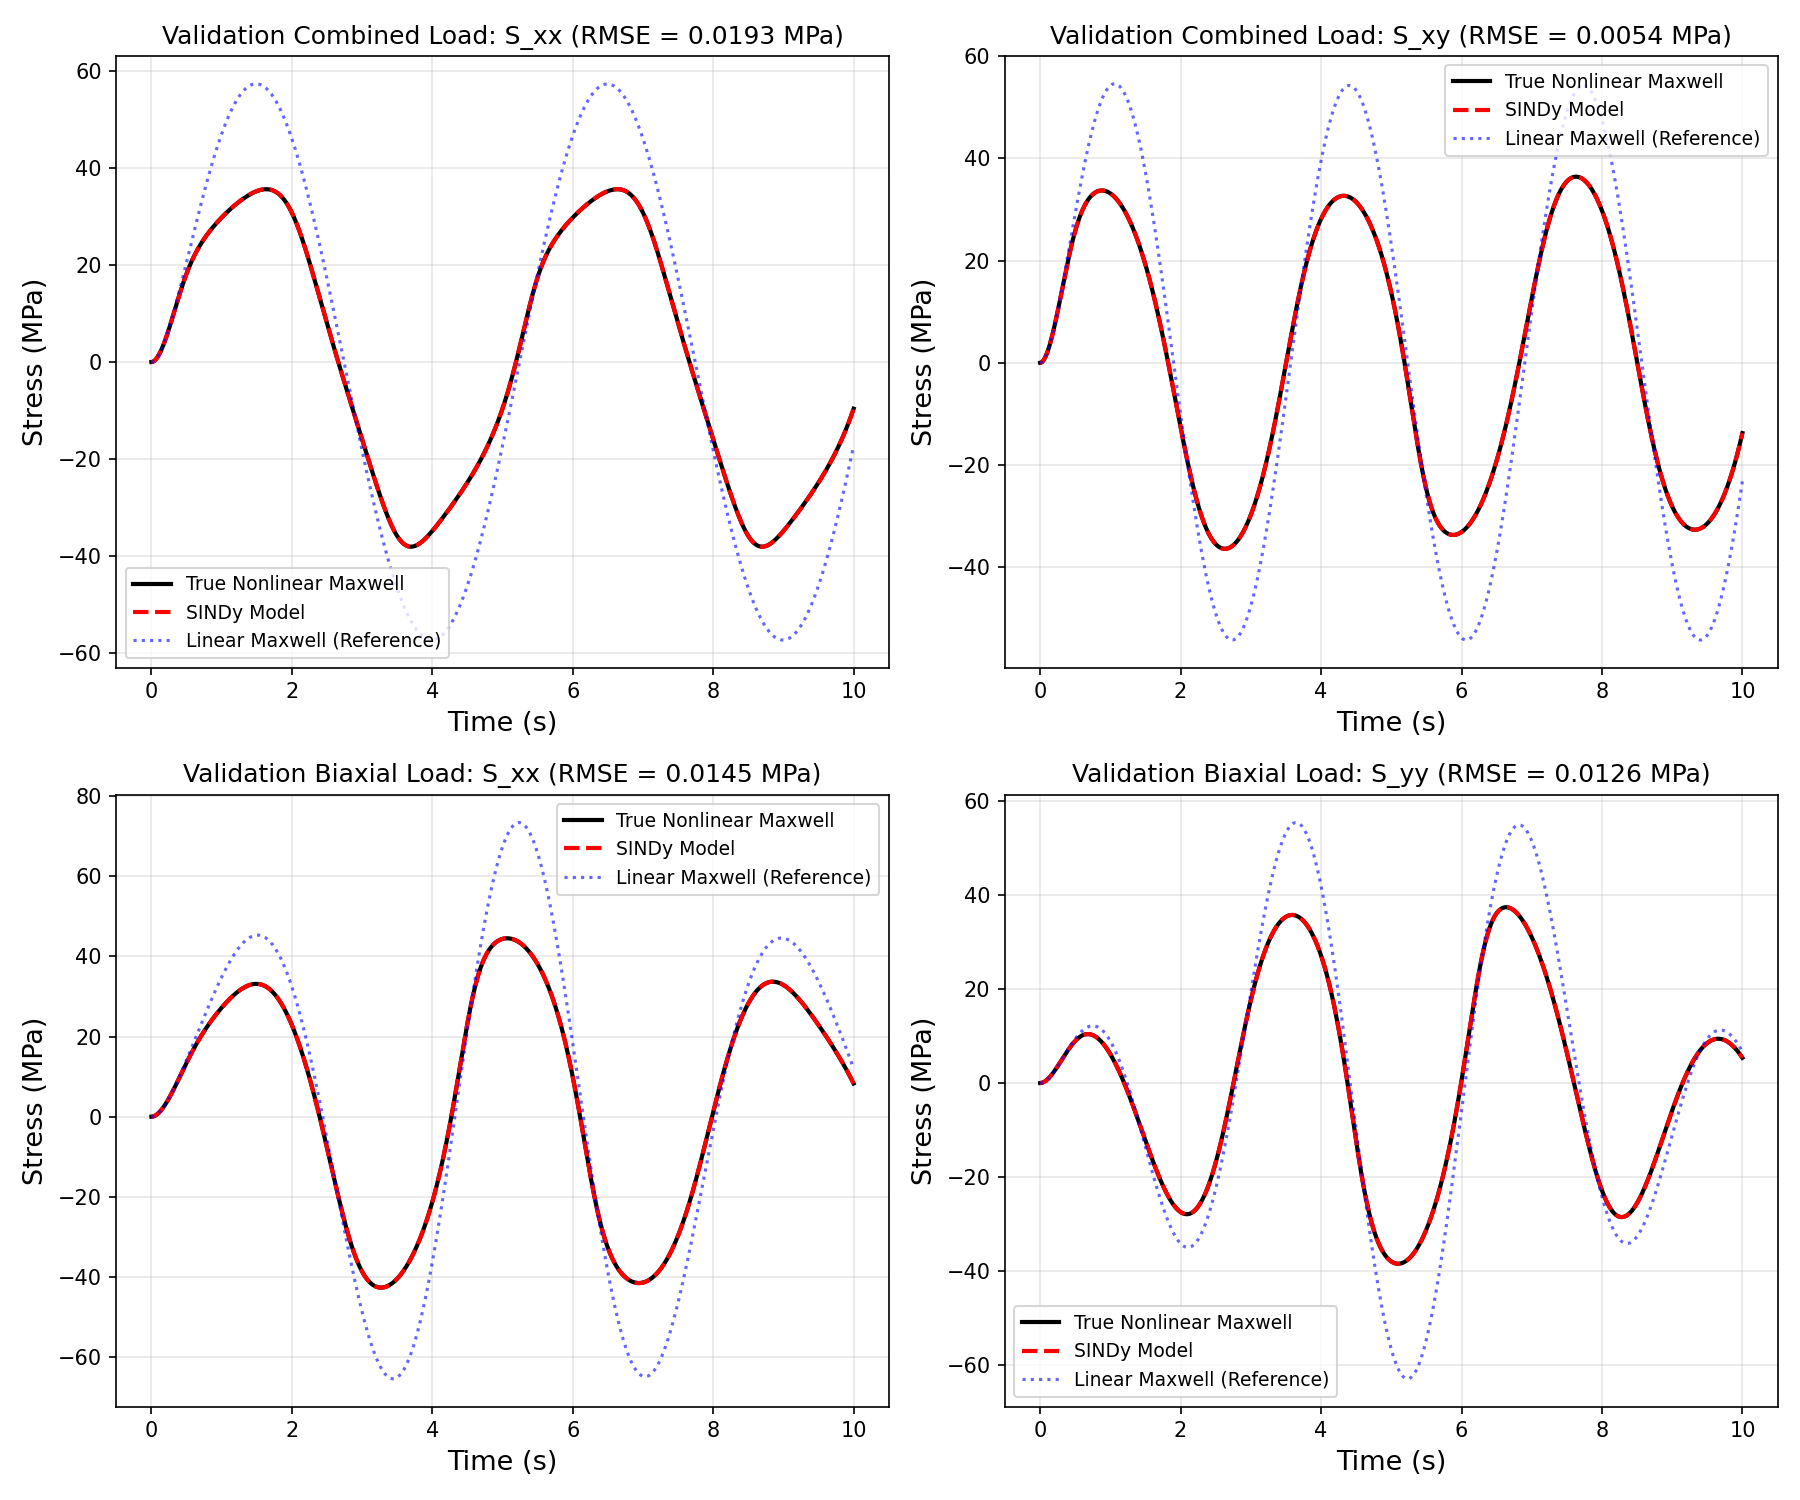
\includegraphics[width=\textwidth]{plot.png}
    \caption{Validation comparison showing True Nonlinear Maxwell response (solid black line), SINDy model predictions (dashed red line), and Linear Maxwell model reference predictions (dotted blue line) across the Combined and Biaxial validation loading trajectories.}
    \label{fig:validation_plot}
\end{figure}

\end{document}
